% =========================
% chapter1.tex
% =========================

\chapter{Metodyka badań: dane, przetwarzanie i modele}

\section{Charakterystyka źródeł danych i struktura zbiorów}

Podstawę materiałową badań stanowiły ogólnodostępne zbiory danych treningowych kolarstwa szosowego, zgromadzone w ramach inicjatyw typu \textit{Open Science} oraz repozytoriów dla analizy danych sportowych.
Wybór gotowych, zanonimizowanych zbiorów danych podyktowany był koniecznością zapewnienia dużej różnorodności próby badawczej (różny poziom wytrenowania, wiek i płeć zawodników), co jest kluczowe dla zdolności generalizacji modeli uczenia maszynowego \cite{stockwell2023mlftp}.

W badaniu wykorzystano dwa główne źródła danych:
\begin{enumerate}
  \item \textbf{GoldenCheetah OpenData} - wielkoskalowe repozytorium zawierające tysiące plików treningowych udostępnionych przez użytkowników oprogramowania GoldenCheetah.
  Zbiór ten charakteryzuje się wysoką różnorodnością warunków treningowych (jazda tlenowa, interwały, wyścigi), odzwierciedlając rzeczywiste scenariusze użytkowania mierników mocy w terenie \cite{kaggle_cycling_data}.
  \item \textbf{Zbiór referencyjny} - uzupełniający zestaw danych zawierający wyniki ustrukturyzowanych testów wydolnościowych (np.\ protokoły testów rampowych lub testy czasowe), który posłużył do walidacji metodyki wyznaczania wartości referencyjnych \cite{figshare_cycling_data}.
\end{enumerate}

Podstawę analizy stanowił obszerny zbiór danych treningowych pochodzący z repozytorium GoldenCheetah OpenData oraz uzupełniający zbiór referencyjny. Do eksperymentu wyselekcjonowano reprezentatywną grupę zawodników, których historia treningowa spełniała rygorystyczne kryteria jakościowe dotyczące ciągłości zapisu mocy i tętna, zdefiniowane w dalszej części rozdziału.
\subsection{Struktura szeregów czasowych}

Dane wejściowe mają postać wielowymiarowych szeregów czasowych.
Każda sesja treningowa zapisana jest w formacie (np.\ $\mathrm{CSV}$ lub $\mathrm{FIT}$), gdzie pojedynczy wiersz odpowiada jednej próbce pomiarowej.
Zgodnie ze standardem urządzeń rejestrujących (np.\ liczniki rowerowe Garmin, Wahoo), częstotliwość próbkowania wynosi $1\ \mathrm{Hz}$.

Dla każdego punktu w czasie $t$ dostępny jest wektor cech $\mathbf{x}_t$ zawierający m.in.:
\begin{itemize}
  \item \textbf{Moc} ($P$) - chwilowa moc mechaniczna generowana przez zawodnika, wyrażona w watach [$\mathrm{W}$]. Jest to główna zmienna niezależna (sygnał wejściowy) \cite{allen2019power}.
  \item \textbf{Tętno} ($HR$) - częstość skurczów serca wyrażona w uderzeniach na minutę [$\mathrm{bpm}$]. Stanowi zmienną opisującą odpowiedź fizjologiczną organizmu na zadane obciążenie \cite{borszcz2018ftp,sitko2022tte}.
  \item \textbf{Kadencja} ($CAD$) - rytm pedałowania w obrotach na minutę [$\mathrm{rpm}$], wykorzystywany pomocniczo do detekcji przerw w jeździe (tzw.\ \textit{coasting}).
  \item \textbf{Znacznik czasu} - umożliwia rekonstrukcję chronologii zdarzeń i obliczanie cech pochodnych w dziedzinie czasu.
\end{itemize}

Dodatkowo zbiory danych zawierały metadane dotyczące zawodników, takie jak masa ciała (niezbędna do wyznaczenia współczynnika $\mathrm{W\,kg^{-1}}$) oraz, w wybranych przypadkach, historyczne wartości $\mathrm{FTP}$ deklarowane przez użytkowników, które posłużyły jako punkt odniesienia dla procedury etykietowania \cite{stockwell2023mlftp}.

Ze względu na terenowy charakter rejestracji surowe dane obarczone były szumem pomiarowym, w tym występowaniem wartości pustych (np.\ zaników sygnału z czujników $\mathrm{ANT+}$) oraz artefaktów (np.\ nierealistyczne piki mocy $> 2000\ \mathrm{W}$), co wymusiło zastosowanie procedur czyszczenia opisanych w kolejnym podrozdziale \cite{uspatent2024ftp}.

\section{Wstępne przetwarzanie danych}

Dane surowe rejestrowane w warunkach terenowych obarczone są zakłóceniami wynikającymi ze specyfiki pomiaru (np.\ utrata łączności czujników $\mathrm{ANT+}/\mathrm{Bluetooth}$, błędy kalibracji, zakłócenia GPS) oraz charakterystyki jazdy (postoje, zjazdy).
Bezpośrednie wykorzystanie takich szeregów czasowych w modelach uczenia maszynowego prowadziłoby do niestabilności uczenia i obniżenia zdolności generalizacji \cite{stockwell2023mlftp}.

Przed ekstrakcją cech zastosowano wieloetapową procedurę czyszczenia i normalizacji danych.

\subsection{Filtracja artefaktów i wartości niefizjologicznych}

W pierwszej kolejności usunięto obserwacje zawierające błędy grube, definiowane jako wartości wykraczające poza biologiczne lub mechaniczne możliwości układu kolarz--rower.
Na podstawie literatury przedmiotu oraz analizy rozkładu zmiennych w zbiorze treningowym przyjęto następujące filtry progowe:
\begin{itemize}
  \item \textbf{Moc} ($P$): wartości $P > 2000\ \mathrm{W}$ uznano za błędy pomiarowe i zastąpiono wartością \texttt{NaN}, a następnie poddano interpolacji. Usunięto również wartości ujemne.
  \item \textbf{Tętno} ($HR$): za zakres fizjologiczny uznano przedział $30 \le HR \le 220\ \mathrm{bpm}$.
  \item \textbf{Kadencja} ($CAD$): wartości $CAD > 200\ \mathrm{rpm}$ uznano za artefakty i odfiltrowano.
\end{itemize}

\subsection{Ciągłość danych i interpolacja}

Standardowe pliki treningowe (formaty \texttt{.fit}/\texttt{.gpx}) często nie zachowują stałej częstotliwości próbkowania w przypadku utraty sygnału lub włączenia funkcji \textit{auto-pause}.
Aby umożliwić analizę w domenie częstotliwości oraz poprawne wyliczanie średnich kroczących, wszystkie szeregi czasowe zostały poddane resamplingowi do stałej częstotliwości $1\ \mathrm{Hz}$.

Brakujące próbki uzupełniano w zależności od długości przerwy:
\begin{enumerate}
  \item \textbf{Krótkie przerwy} ($\Delta t < 5\ \mathrm{s}$): interpolacja liniowa.
  \item \textbf{Długie przerwy} ($\Delta t \ge 5\ \mathrm{s}$): pozostawiano jako braki danych lub (w przypadku postojów) wypełniano zerami dla mocy i kadencji w celu poprawnego odwzorowania obciążenia.
\end{enumerate}

\subsection{Obsługa postojów i segmentacja}

W analizie danych z jazdy swobodnej istotnym wyzwaniem jest obecność fragmentów, w których zawodnik nie pedałuje (zjazdy, dojazd do skrzyżowań).
W procedurze przetwarzania przyjęto rozróżnienie na:
\begin{itemize}
  \item \textbf{czas całkowity} - od startu do zatrzymania rejestracji,
  \item \textbf{czas ruchu} - czas, w którym $v > 0$ lub $P > 0$.
\end{itemize}

Dla potrzeb inżynierii cech (np.\ obliczania mocy znormalizowanej, $\mathrm{NP}$) uwzględniono zera w sygnale mocy (zjazdy), ponieważ stanowią element regeneracji w trakcie wysiłku interwałowego.
Okresy długotrwałego postoju (powyżej 30 s) niezwiązane z procesem treningowym wyłączono z analizy, aby zachować reprezentatywność średnich parametrów fizjologicznych.

\subsection{Kryteria selekcji sesji}

Ostatnim etapem preprocessingu była selekcja jednostek treningowych przydatnych do uczenia modelu.
Ze zbioru danych usunięto sesje niespełniające minimalnych kryteriów jakościowych:
\begin{itemize}
  \item czas trwania krótszy niż 30 minut,
  \item brak pełnego zapisu tętna,
  \item wysoki odsetek brakujących danych (powyżej 10\%).
\end{itemize}

\section{Definicja zmiennej celu}

W paradygmacie uczenia nadzorowanego niezbędne jest przypisanie każdej obserwacji wejściowej $X$ (sesja treningowa) odpowiadającej jej etykiety $y$ (rzeczywista wartość $\mathrm{FTP}$).
Ponieważ standardowe pliki treningowe nie zawierają jawnej informacji o aktualnym progu mocy, a testy wydolnościowe wykonywane są nieregularnie, zastosowano heurystyczny algorytm etykietowania oparty na detekcji wysiłków maksymalnych oraz propagacji czasowej.

\subsection{Wyznaczanie wartości referencyjnych FTP}

Jako punkt wyjścia przyjęto definicję funkcjonalną, zgodnie z którą estymator $\mathrm{FTP}$ można wyznaczyć na podstawie $20$-minutowego wysiłku maksymalnego ($\mathrm{MMP}_{20\ \mathrm{min}}$).

Dla każdego zawodnika zanalizowano historię treningów, identyfikując sesje zawierające potencjalne próby testowe.
Wartość referencyjną $\mathrm{FTP}_{\mathrm{ref}}^{(i)}$ dla sesji testowej $i$ wyznaczano zgodnie ze wzorem:
\begin{equation}
\label{eq:ftp_ref_mmp20}
\mathrm{FTP}_{\mathrm{ref}}^{(i)} = 0.95 \cdot \max\!\left(\overline{P}_{20\ \mathrm{min}}(t)\right),
\end{equation}
gdzie $\max(\overline{P}_{20\ \mathrm{min}}(t))$ oznacza najwyższą średnią moc kroczącą z $20$-minutowego okna zarejestrowaną w trakcie danej jednostki treningowej.

Aby uniknąć błędnego etykietowania na podstawie przypadkowych, niemaksymalnych wysiłków, jako wiarygodne punkty odniesienia traktowano tylko wyniki stanowiące lokalne maksima w historii zawodnika lub wyraźnie oznaczone w metadanych (jeśli dostępne).

\subsection{Strategia propagacji etykiet}

Wydolność tlenowa jest parametrem wolnozmiennym, dlatego przyjęto założenie o przybliżonej stacjonarności $\mathrm{FTP}$ w krótkim oknie czasowym.
Do stworzenia zbioru uczącego etykiety z punktów testowych propagowano do sąsiednich sesji treningowych w symetrycznym oknie czasowym $\Delta t = \pm 14$ dni.

Procedurę przypisywania etykiety $y_j$ dla sesji treningowej $j$ odbywającej się w czasie $t_j$ zdefiniowano następująco:
\begin{enumerate}
  \item Zidentyfikowano najbliższy w czasie wiarygodny test referencyjny wykonany w czasie $t_{\mathrm{test}}$.
  \item Sprawdzono warunek odległości czasowej:
  \[
    \left|t_j - t_{\mathrm{test}}\right| \le 14\ \text{dni}.
  \]
  \item W przypadku spełnienia warunku przypisano:
  \[
    y_j = \mathrm{FTP}_{\mathrm{ref}}(t_{\mathrm{test}}).
  \]
\end{enumerate}

W sytuacjach konfliktowych, gdy sesja znajdowała się w zasięgu dwóch testów, przypisywano wartość z testu bliższego chronologicznie.
Sesje bez testu referencyjnego w zadanym oknie wyłączono ze zbioru uczącego.

\begin{figure}[htbp]
  \centering
  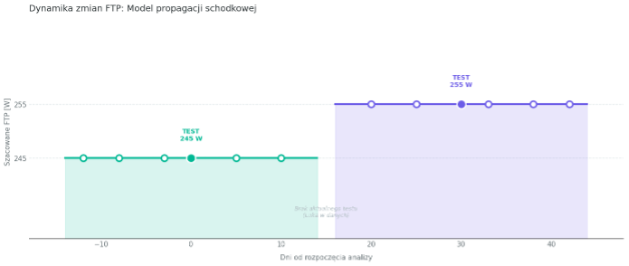
\includegraphics[width=0.95\linewidth]{figures/fig5_label_propagation_ftp_over_time.png}
  \caption{Przebieg zmienności estymowanego $\mathrm{FTP}$ w czasie. Model zakłada stałość parametru (poziome odcinki) w oknie ważności testu, z aktualizacją wartości po wykonaniu nowego testu referencyjnego. Źródło: Opracowanie własne.}
  \label{fig:label_propagation_ftp}
\end{figure}

\section{Inżynieria cech}

Surowe szeregi czasowe mają wymiarowość zależną od czasu trwania treningu, natomiast większość klasycznych algorytmów uczenia maszynowego wymaga wejścia o stałym wymiarze.
Z tego powodu przeprowadzono ekstrakcję cech, której celem była transformacja zmiennych czasowych w zestaw zagregowanych predyktorów opisujących charakterystykę wysiłku oraz odpowiedź fizjologiczną organizmu.

Ostateczny wektor wejściowy $\mathbf{X}$ dla każdej sesji zawierał 28 cech, pogrupowanych w trzy główne kategorie.

\subsection{Statystyczne agregaty parametrów wysiłkowych}

Dla sygnałów mocy ($P$) i tętna ($HR$) wyznaczono m.in.:
\begin{itemize}
  \item średnie arytmetyczne ($P_{\mathrm{avg}}$, $HR_{\mathrm{avg}}$),
  \item maksima oraz percentyle (np.\ $95$.\ percentyl),
  \item odchylenia standardowe ($\sigma_P$, $\sigma_{HR}$) jako miary zmienności sygnału.
\end{itemize}

\subsection{Zaawansowane wskaźniki domenowe}

Ze względu na nieliniowy charakter zmęczenia mięśniowego uwzględniono specjalistyczne wskaźniki ze sportometrii.

\paragraph{Moc znormalizowana (NP).}
Zgodnie z algorytmem Coggana, $\mathrm{NP}$ wyznacza się poprzez wygładzenie sygnału mocy średnią kroczącą z okna $30\ \mathrm{s}$, podniesienie do potęgi czwartej, uśrednienie i spierwiastkowanie:
\begin{equation}
\label{eq:np_definition}
\mathrm{NP} = \left(\frac{1}{n}\sum_{i=1}^{n} \left(\overline{P}_{30\ \mathrm{s}}(i)\right)^{4}\right)^{\frac{1}{4}}.
\end{equation}
\cite{allen2019power}

\paragraph{Maksymalne średnie z okien czasowych (MMP).}
Wyznaczono maksymalne średnie moce z okien: $1$ min, $5$ min oraz $20$ min (profil mocy).

\paragraph{Stosunek mocy do tętna (EF).}
Wskaźnik \textit{Efficiency Factor} zdefiniowano jako:
\begin{equation}
\label{eq:ef_definition}
\mathrm{EF} = \frac{\mathrm{NP}}{HR_{\mathrm{avg}}},
\end{equation}
alternatywnie w uproszczeniu $\mathrm{EF}=\frac{P_{\mathrm{avg}}}{HR_{\mathrm{avg}}}$.

\subsection{Kwantyzacja intensywności}

Aby uniknąć zależności cyrkularnej i ryzyka \textit{data leakage} (strefy mocy oparte na \% $\mathrm{FTP}$), zastosowano bezwzględne koszyki mocy o stałej szerokości.
Utworzono histogram czasu w przedziałach:
\begin{itemize}
  \item moc: koszyki co $50\ \mathrm{W}$ (np.\ $0$--$50$, $50$--$100$, \dots, $>400\ \mathrm{W}$),
  \item tętno: koszyki co $10\ \mathrm{bpm}$ (np.\ $<100$, $100$--$110$, \dots, $>180\ \mathrm{bpm}$).
\end{itemize}
Cechami wejściowymi były znormalizowane udziały czasu spędzone w każdym koszyku.

\subsection{Wskaźniki dryfu tętna}

Aby zidentyfikować efekt dryfu tętna, wyliczono wskaźnik odsprzężenia ($Pw\!:\!HR$).
Sesję dzielono na dwie równe połowy, po czym porównywano stosunek mocy do tętna:
\begin{equation}
\label{eq:decoupling}
\mathrm{Decoupling} =
\frac{\left(\frac{P}{HR}\right)_1 - \left(\frac{P}{HR}\right)_2}{\left(\frac{P}{HR}\right)_1}\cdot 100\%.
\end{equation}

\section{Architektura systemu eksperymentalnego}

Proces trenowania i walidacji modeli osadzono w sformalizowanym potoku eksperymentalnym.
Kluczowym wyzwaniem jest ryzyko wycieku informacji, które może prowadzić do zawyżenia wyników.

\subsection{Strategia podziału zbioru danych}

Losowy podział danych byłby metodologicznie błędny dla szeregów czasowych, szczególnie że treningi zawodnika wykazują silną autokorelację czasową. Zastosowano zatem podział chronologiczny z grupowaniem obserwacji po zawodnikach.
Zbiór danych podzielono na:
\begin{enumerate}
  \item zbiór treningowy (ok.\ $70\%$),
  \item zbiór walidacyjny (ok.\ $15\%$),
  \item zbiór testowy (ok.\ $15\%$), obejmujący sesje z najpóźniejszego okresu.
\end{enumerate}

\subsection{Metryki oceny jakości predykcji}

Do ewaluacji modeli wybrano metryki standardowo stosowane w regresji:
$\mathrm{RMSE}$, $\mathrm{MAE}$ oraz $R^2$ (por.\ równania \ref{eq:rmse}--\ref{eq:r2} w Rozdziale~1) \cite{hastie2009esl,james2021isl,nvidia_regression_metrics}.

\section{Wybrane algorytmy uczenia maszynowego}

W eksperymencie porównano skuteczność trzech klas algorytmów regresyjnych.

\subsection{Regresja liniowa z regularyzacją}

Model liniowy przewiduje wartość:
\begin{equation}
\label{eq:linear_pred}
\hat{y}_i = w_0 + \sum_{j=1}^{p} w_j x_{ij},
\end{equation}
gdzie $x_{ij}$ oznacza wartość $j$-tej cechy dla $i$-tej sesji.

Ze względu na współliniowość cech zastosowano regularyzację $\ell_2$:
\begin{equation}
\label{eq:ridge_objective}
J(\mathbf{w}) = \sum_{i=1}^{n}\left(y_i - \hat{y}_i\right)^2 + \lambda \sum_{j=1}^{p} w_j^2,
\end{equation}
gdzie $\lambda$ jest hiperparametrem sterującym siłą regularyzacji \cite{hastie2009esl}.

\subsection{Random Forest}

Algorytm Lasu Losowego buduje zespół $B$ drzew decyzyjnych trenowanych na losowych próbach bootstrap.
Predykcja zespołu jest średnią predykcji drzew:
\begin{equation}
\label{eq:rf_pred}
\hat{f}_{\mathrm{RF}}(x) = \frac{1}{B}\sum_{b=1}^{B} T_b(x).
\end{equation}
\cite{james2021isl,sanjaykumar2024athlete}

\subsection{XGBoost}

W modelu wzmacniania gradientowego predykcja jest aktualizowana addytywnie:
\begin{equation}
\label{eq:xgb_update}
\hat{y}_i^{(t)} = \hat{y}_i^{(t-1)} + f_t(x_i).
\end{equation}

W XGBoost funkcję celu aproksymuje się rozwinięciem Taylora drugiego rzędu i stosuje regularyzację złożoności drzewa:
\begin{equation}
\label{eq:xgb_objective}
\mathcal{L}^{(t)} \approx
\sum_{i=1}^{n}\left[l\!\left(y_i,\hat{y}_i^{(t-1)}\right) + g_i f_t(x_i) + \frac{1}{2}h_i f_t^2(x_i)\right] + \Omega(f_t),
\end{equation}
gdzie $g_i$ i $h_i$ oznaczają odpowiednio gradient i hesjan funkcji straty względem $\hat{y}$, a $\Omega(\cdot)$ penalizuje złożoność drzewa \cite{stockwell2023mlftp}.

\section{Środowisko implementacji i narzędzia informatyczne}

Całość procesu badawczego (ETL, inżynieria cech, trening i ewaluacja modeli) zaimplementowano w języku Python.
Wybór ten wynika z dominującej roli Pythona w analizie danych oraz dostępności dojrzałych bibliotek naukowych.

\subsection{Język programowania Python}

Projekt zrealizowano w oparciu o interpreter Pythona w wersji $3.10$.
Python, dzięki ekosystemowi bibliotek, umożliwia szybkie prototypowanie oraz efektywne obliczenia wektorowe.

\subsection{Biblioteki do przetwarzania i analizy danych}

Warstwę ETL oparto o NumPy i Pandas:
\begin{itemize}
  \item \textbf{NumPy} - operacje na tablicach wielowymiarowych i obliczenia numeryczne,
  \item \textbf{Pandas} - struktury \texttt{DataFrame} oraz mechanizmy pracy z czasem, m.in.\ \texttt{DatetimeIndex}, \texttt{.resample()}, \texttt{.rolling()}.
\end{itemize}

\subsection{Biblioteki uczenia maszynowego}

Modelowanie predykcyjne zrealizowano z wykorzystaniem Scikit-Learn oraz \textit{XGBoost}:
\begin{itemize}
  \item \textbf{Scikit-Learn} - podział danych (np.\ \texttt{TimeSeriesSplit}, \texttt{GroupKFold}), normalizacja (np.\ \texttt{StandardScaler}), modele bazowe oraz pipeline'y,
  \item \textbf{XGBoost} - algorytm \textit{gradient boosting} z regularyzacją i obsługą braków danych.
\end{itemize}

\subsection{Wizualizacja i środowisko pracy}

Do eksploracyjnej analizy danych i prezentacji wyników wykorzystano Matplotlib oraz Seaborn.
Kod rozwijano w środowisku Jupyter Notebook, co ułatwia łączenie narracji, kodu i wizualizacji.

\section{Podsumowanie}

W niniejszym rozdziale zdefiniowano kompletny proces badawczy.
Dane pozyskane z otwartych repozytoriów poddano czyszczeniu i agregacji, transformując surowe szeregi czasowe w wektory cech opisujące charakterystykę wysiłku.
Zdefiniowano metodę etykietowania opartą na propagacji wyników testów referencyjnych oraz ustalono zasady walidacji chronologicznej.
Tak przygotowane środowisko eksperymentalne stanowi podstawę do badań właściwych, których wyniki zostaną zaprezentowane w kolejnych rozdziałach.